% =====================================================================
% Fig. 2 - Multiscale Decomposition (FEATHer module [1]). v3.
%
% Design changes from v2:
%   - Branch name + kernel size fused into the operator block itself
%     (no separate label column overlapping the input box).
%   - Wider lateral spacing so arrows have visible heads.
%   - Equations omitted; they live in the methodology text.
% =====================================================================
\documentclass[tikz, border=8pt]{standalone}

\usepackage{amsmath, amssymb}
\usepackage{tikz}
\usetikzlibrary{arrows.meta, positioning, calc, decorations.pathreplacing}

\definecolor{pointC}{HTML}{6B7280}
\definecolor{highC}{HTML}{DC2626}
\definecolor{midC}{HTML}{F59E0B}
\definecolor{lowC}{HTML}{2563EB}

\begin{document}

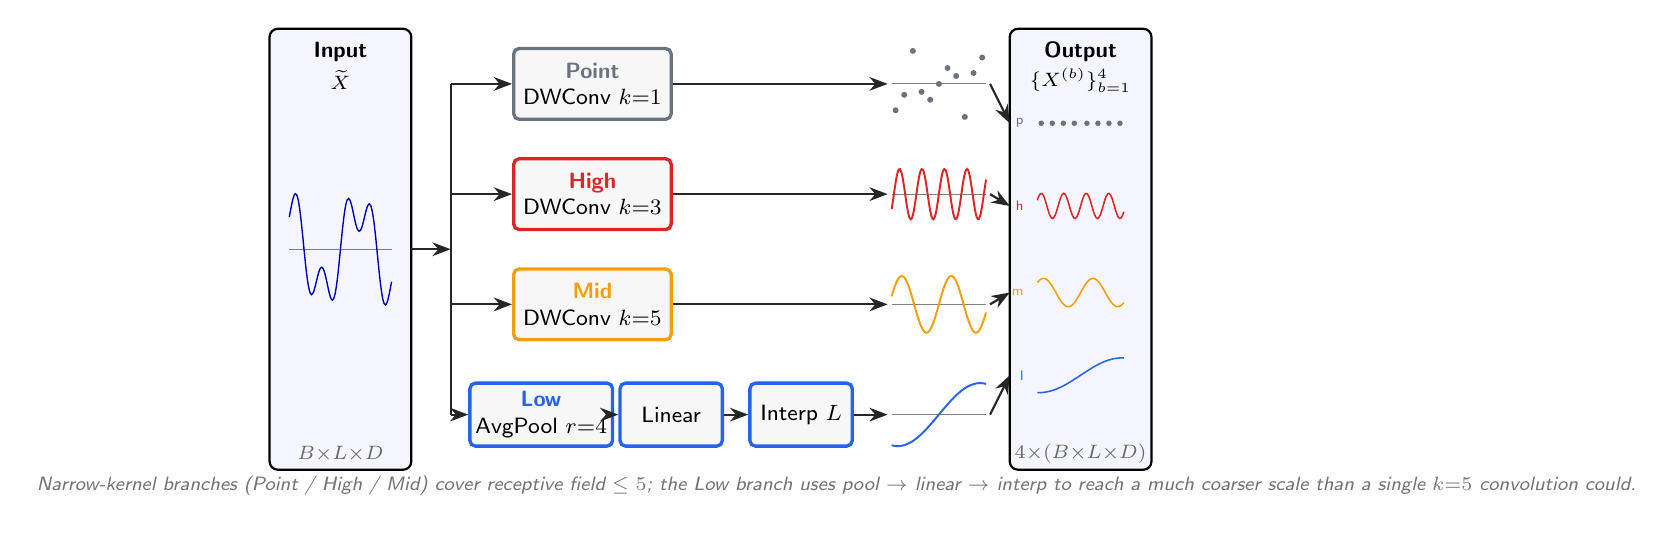
\begin{tikzpicture}[
    font=\sffamily\small,
    >=Stealth,
    op/.style={
        draw, thick,
        rounded corners=2pt,
        fill=gray!6,
        minimum width=2.0cm,
        minimum height=0.9cm,
        align=center,
        font=\sffamily\footnotesize,
        inner sep=2pt
    },
    smallop/.style={
        draw, thick,
        rounded corners=2pt,
        fill=gray!6,
        minimum width=1.3cm,
        minimum height=0.8cm,
        align=center,
        font=\sffamily\footnotesize,
        inner sep=2pt
    },
    iobox/.style={
        draw, thick,
        rounded corners=3pt,
        fill=blue!4,
        minimum width=1.8cm,
        minimum height=5.6cm
    },
    flow/.style={->, thick, draw=black!85},
    axis/.style={draw=black!50, line width=0.3pt}
]

% =====================================================================
% Geometry
% =====================================================================
\def\inX{0}
\def\splitX{1.4}
\def\opX{3.2}            % single-op center x (point/high/mid)
% Low branch ops well-separated to keep arrow heads visible
\def\lowAx{2.55}
\def\lowBx{4.20}
\def\lowCx{5.85}
\def\wfX{7.6}
\def\outX{9.4}

\def\yP{2.1}
\def\yH{0.7}
\def\yM{-0.7}
\def\yL{-2.1}

% =====================================================================
% Input container
% =====================================================================
\node[iobox] (INBOX) at (\inX, 0) {};
\node[font=\sffamily\bfseries\footnotesize] at (\inX, 2.5) {Input};
\node[font=\sffamily\scriptsize] at (\inX, 2.15) {$\widetilde{X}$};
\node[font=\sffamily\scriptsize, text=black!60] at (\inX, -2.6) {$B{\times}L{\times}D$};
\begin{scope}[shift={(\inX, 0)}]
    \draw[axis] (-0.65, 0) -- (0.65, 0);
    \draw[blue!70!black, line width=0.5pt, smooth, samples=70, domain=-0.65:0.65]
        plot (\x, {0.55*sin(7*\x r) + 0.32*sin(20*\x r)});
\end{scope}

% =====================================================================
% Operator blocks (branch label + operator fused)
% =====================================================================
\node[op, draw=pointC, very thick] (OPp) at (\opX, \yP) {%
    \textcolor{pointC}{\textbf{Point}}\\ DWConv $k{=}1$};
\node[op, draw=highC, very thick]  (OPh) at (\opX, \yH) {%
    \textcolor{highC}{\textbf{High}}\\ DWConv $k{=}3$};
\node[op, draw=midC, very thick]   (OPm) at (\opX, \yM) {%
    \textcolor{midC}{\textbf{Mid}}\\ DWConv $k{=}5$};

% Low branch chain
\node[smallop, draw=lowC, very thick] (OPla) at (\lowAx, \yL) {%
    \textcolor{lowC}{\textbf{Low}}\\ AvgPool $r{=}4$};
\node[smallop, draw=lowC, very thick] (OPlb) at (\lowBx, \yL) {Linear};
\node[smallop, draw=lowC, very thick] (OPlc) at (\lowCx, \yL) {Interp $L$};

% =====================================================================
% Branch output mini-waveforms
% =====================================================================
\begin{scope}[shift={(\wfX, \yP)}]
    \draw[axis] (-0.6, 0) -- (0.6, 0);
    \foreach \xi in {-0.55, -0.44, -0.33, -0.22, -0.11, 0, 0.11, 0.22, 0.33, 0.44, 0.55} {
        \fill[pointC] (\xi, {0.30*sin(15*\xi r) + 0.15*sin(35*\xi r)}) circle (0.038);
    }
\end{scope}
\begin{scope}[shift={(\wfX, \yH)}]
    \draw[axis] (-0.6, 0) -- (0.6, 0);
    \draw[highC, line width=0.7pt, smooth, samples=80, domain=-0.6:0.6]
        plot (\x, {0.32*sin(22*\x r)});
\end{scope}
\begin{scope}[shift={(\wfX, \yM)}]
    \draw[axis] (-0.6, 0) -- (0.6, 0);
    \draw[midC, line width=0.7pt, smooth, samples=80, domain=-0.6:0.6]
        plot (\x, {0.36*sin(10*\x r)});
\end{scope}
\begin{scope}[shift={(\wfX, \yL)}]
    \draw[axis] (-0.6, 0) -- (0.6, 0);
    \draw[lowC, line width=0.7pt, smooth, samples=80, domain=-0.6:0.6]
        plot (\x, {0.40*sin(3*\x r)});
\end{scope}

% =====================================================================
% Output container with 4 stacked mini-waveforms
% =====================================================================
\node[iobox] (OUTBOX) at (\outX, 0) {};
\node[font=\sffamily\bfseries\footnotesize] at (\outX, 2.5) {Output};
\node[font=\sffamily\scriptsize] at (\outX, 2.15) {$\{X^{(b)}\}_{b=1}^{4}$};
\node[font=\sffamily\scriptsize, text=black!60] at (\outX, -2.6) {$4{\times}(B{\times}L{\times}D)$};

\begin{scope}[shift={(\outX, 0)}]
    \def\wW{0.55}
    \foreach \xi in {-0.50, -0.36, -0.22, -0.08, 0.08, 0.22, 0.36, 0.50} {
        \fill[pointC] (\xi, 1.6) circle (0.035);
    }
    \node[font=\sffamily\tiny, text=pointC, anchor=east] at (-\wW - 0.05, 1.6) {p};
    \draw[highC, line width=0.55pt, smooth, samples=60, domain=-\wW:\wW]
        plot (\x, {0.55 + 0.16*sin(22*\x r)});
    \node[font=\sffamily\tiny, text=highC, anchor=east] at (-\wW - 0.05, 0.55) {h};
    \draw[midC, line width=0.55pt, smooth, samples=60, domain=-\wW:\wW]
        plot (\x, {-0.55 + 0.18*sin(10*\x r)});
    \node[font=\sffamily\tiny, text=midC, anchor=east] at (-\wW - 0.05, -0.55) {m};
    \draw[lowC, line width=0.55pt, smooth, samples=60, domain=-\wW:\wW]
        plot (\x, {-1.6 + 0.22*sin(3*\x r)});
    \node[font=\sffamily\tiny, text=lowC, anchor=east] at (-\wW - 0.05, -1.6) {l};
\end{scope}

% =====================================================================
% Arrows
% =====================================================================
% input box -> fan-out
\draw[flow] (\inX + 0.9, 0) -- (\splitX, 0);
% vertical fan-out bus
\draw[draw=black!85, thick] (\splitX, \yP) -- (\splitX, \yL);
% bus -> each operator
\draw[flow] (\splitX, \yP) -- (OPp.west);
\draw[flow] (\splitX, \yH) -- (OPh.west);
\draw[flow] (\splitX, \yM) -- (OPm.west);
\draw[flow] (\splitX, \yL) -- (OPla.west);

% within Low chain
\draw[flow] (OPla.east) -- (OPlb.west);
\draw[flow] (OPlb.east) -- (OPlc.west);

% operator -> mini-waveform
\draw[flow] (OPp.east)  -- (\wfX - 0.65, \yP);
\draw[flow] (OPh.east)  -- (\wfX - 0.65, \yH);
\draw[flow] (OPm.east)  -- (\wfX - 0.65, \yM);
\draw[flow] (OPlc.east) -- (\wfX - 0.65, \yL);

% mini-waveform -> output box (converge)
\draw[flow] (\wfX + 0.65, \yP) -- (\outX - 0.9,  1.6);
\draw[flow] (\wfX + 0.65, \yH) -- (\outX - 0.9,  0.55);
\draw[flow] (\wfX + 0.65, \yM) -- (\outX - 0.9, -0.55);
\draw[flow] (\wfX + 0.65, \yL) -- (\outX - 0.9, -1.6);

% =====================================================================
% Bottom annotation: R5 #5 defense (asymmetric Low branch)
% =====================================================================
\node[font=\sffamily\scriptsize\itshape, text=black!55, align=center]
    at ({(\opX + \outX)/2}, -3.0)
    {Narrow-kernel branches (Point / High / Mid) cover receptive field $\le 5$;
     the Low branch uses pool $\to$ linear $\to$ interp to reach a much coarser scale
     than a single $k{=}5$ convolution could.};

\end{tikzpicture}

\end{document}
